\begin{figure}[H]
    \centering
    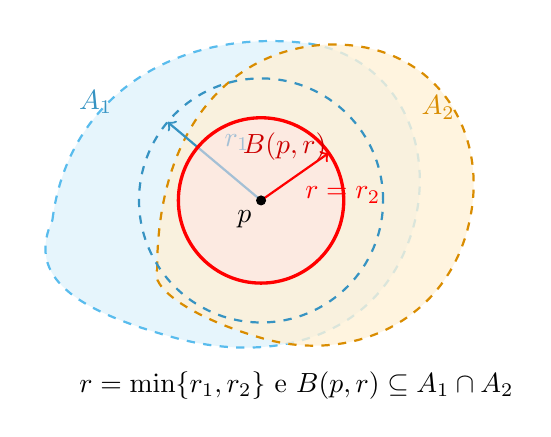
\begin{tikzpicture}[scale=1.0]
        % Aberto A_1.
        \path[fill=Cerulean!12, fill opacity=0.85]
            (-2.65,-0.25)
            .. controls (-2.45,1.35) and (-1.05,2.18) .. (0.55,2.00)
            .. controls (1.70,1.86) and (2.28,0.70) .. (1.90,-0.45)
            .. controls (1.45,-1.78) and (0.10,-2.10) .. (-1.18,-1.72)
            .. controls (-2.50,-1.35) and (-2.95,-0.90) .. (-2.65,-0.25)
            -- cycle;
        \draw[Cerulean!70, thick, dashed]
            (-2.65,-0.25)
            .. controls (-2.45,1.35) and (-1.05,2.18) .. (0.55,2.00)
            .. controls (1.70,1.86) and (2.28,0.70) .. (1.90,-0.45)
            .. controls (1.45,-1.78) and (0.10,-2.10) .. (-1.18,-1.72)
            .. controls (-2.50,-1.35) and (-2.95,-0.90) .. (-2.65,-0.25)
            -- cycle;

        % Aberto A_2.
        \path[fill=Orange!16, fill opacity=0.78]
            (-1.32,-0.88)
            .. controls (-1.32,0.92) and (-0.38,1.93) .. (0.85,1.98)
            .. controls (2.18,2.02) and (2.88,0.92) .. (2.66,-0.20)
            .. controls (2.42,-1.48) and (1.22,-2.08) .. (0.05,-1.76)
            .. controls (-0.94,-1.48) and (-1.42,-1.08) .. (-1.32,-0.88)
            -- cycle;
        \draw[Orange!85!black, thick, dashed]
            (-1.32,-0.88)
            .. controls (-1.32,0.92) and (-0.38,1.93) .. (0.85,1.98)
            .. controls (2.18,2.02) and (2.88,0.92) .. (2.66,-0.20)
            .. controls (2.42,-1.48) and (1.22,-2.08) .. (0.05,-1.76)
            .. controls (-0.94,-1.48) and (-1.42,-1.08) .. (-1.32,-0.88)
            -- cycle;

        \coordinate (p) at (0,0);

        % Bolas fornecidas pela abertura de A_1 e de A_2.
        \draw[Cerulean!80!black, thick, dashed] (p) circle (1.55);
        \draw[Cerulean!80!black, thick, ->] (p) -- ++(140:1.55)
            node[midway, above right] {$r_1$};

        % Neste desenho, r_2 e o menor raio.
        \path[fill=Red!10, fill opacity=0.55] (p) circle (1.05);
        \draw[Red, very thick] (p) circle (1.05);
        \draw[Red, thick, ->] (p) -- ++(35:1.05)
            node[midway, below right] {$r=r_2$};

        \filldraw[black] (p) circle (1.6pt) node[below left] {$p$};

        \node[Cerulean!80!black] at (-2.10,1.25) {$A_1$};
        \node[Orange!85!black] at (2.25,1.18) {$A_2$};
        \node[Red!80!black] at (0.30,0.68) {$B(p,r)$};
        \node at (0.45,-2.35) {$r=\min\{r_1,r_2\}$ e $B(p,r)\subseteq A_1\cap A_2$};
    \end{tikzpicture}
    \caption{Ilustração do item (iii): a menor das bolas centradas em $p$ permanece dentro de $A_1\cap A_2$.}
\end{figure}
